Sketch the solid ellipsoids ${(\textbf{x} - \bar{\textbf{x}})}^{\prime}\textbf{S}^{-1}(\textbf{x} - \bar{\textbf{x}})$ [see (3-16)] for the three matrices
\[
    \textbf{S}
    =
    \begin{bNiceArray}{cc}
        5 & 4 \\
        4 & 5
    \end{bNiceArray}
    ,\hspace{0.2in}
    \textbf{S}
    =
    \begin{bNiceArray}{cc}
        5 & -4 \\
        -4 & 5
    \end{bNiceArray}
    ,\hspace{0.2in}
    \textbf{S}
    =
    \begin{bNiceArray}{cc}
        3 & 0 \\
        0 & 3
    \end{bNiceArray}
\]
(Note that these matrices have the \textit{same} generalized variance $\left|   \textbf{S}\right|$.)
\[
    \textbf{S}
    =
    \begin{bNiceArray}{cc}
        5 & 4 \\
        4 & 5
    \end{bNiceArray}
\]
\[
    0
    =
    \left|\textbf{S} - \lambda \textbf{I}\right|
    =
    \left|
    \begin{NiceArray}{cc}
        5 - \lambda & 4 \\
        4 & 5 - \lambda
    \end{NiceArray}
    \right|
    =
    {(5 - \lambda)}^{2} - 16
    =
    \lambda^2 - 10\lambda + 9
    =
    (\lambda - 9)(\lambda - 1)
\]
The eigenvalues are $\{\lambda_1,\lambda_2\} = \{1,9\}$.
\newline
\underline{$\lambda_1 = 1$:}
\[
    \textbf{S}\textbf{x}_1 = \lambda_1\textbf{x}_1
    \Rightarrow
    \begin{bNiceArray}{cc}
        5 & 4 \\
        4 & 5
    \end{bNiceArray}
    \begin{bNiceArray}{c}
        x_1 \\
        x_2
    \end{bNiceArray}
    =
    \begin{bNiceArray}{c}
        x_1 \\
        x_2
    \end{bNiceArray}
    \Rightarrow
    \begin{bNiceArray}{cc}
        4 & 4 \\
        4 & 4
    \end{bNiceArray}
    \begin{bNiceArray}{c}
        x_1 \\
        x_2
    \end{bNiceArray}
    =
    \begin{bNiceArray}{c}
        0 \\
        0
    \end{bNiceArray}
\]
\[
    \textbf{x}_1
    =
    \begin{bNiceArray}{r}
        1 \\
        -1
    \end{bNiceArray}
    \Rightarrow
    \textbf{e}_1
    =
    \begin{bNiceArray}{r}
        1/\sqrt{2} \\
        -1/\sqrt{2}
    \end{bNiceArray}
\]
\underline{$\lambda_2 = 9$:}
\[
    \textbf{S}\textbf{x}_2 = \lambda_2\textbf{x}_2
    \Rightarrow
    \begin{bNiceArray}{cc}
        5 & 4 \\
        4 & 5
    \end{bNiceArray}
    \begin{bNiceArray}{c}
        x_1 \\
        x_2
    \end{bNiceArray}
    =
    \begin{bNiceArray}{c}
        9x_1 \\
        9x_2
    \end{bNiceArray}
    \Rightarrow
    \begin{bNiceArray}{cc}
        -4 & 4 \\
        4 & -4
    \end{bNiceArray}
    \begin{bNiceArray}{c}
        x_1 \\
        x_2
    \end{bNiceArray}
    =
    \begin{bNiceArray}{c}
        0 \\
        0
    \end{bNiceArray}
\]
\[
    \textbf{x}_2
    =
    \begin{bNiceArray}{c}
        1 \\
        1
    \end{bNiceArray}
    \Rightarrow
    \textbf{e}_2
    =
    \begin{bNiceArray}{c}
        1/\sqrt{2} \\
        1/\sqrt{2}
    \end{bNiceArray}
\]
\[
    \textbf{S}
    =
    \lambda_1
    \textbf{e}_1
    \textbf{e}_1^{\prime}
    +
    \lambda_2
    \textbf{e}_2
    \textbf{e}_2^{\prime}
\]
\[
    \Rightarrow
    \textbf{x}^{\prime}
    \textbf{S}
    \textbf{x}
    =
    \textbf{x}^{\prime}
    \left(
        \lambda_1
        \textbf{e}_1
        \textbf{e}_1^{\prime}
        +
        \lambda_2
        \textbf{e}_2
        \textbf{e}_2^{\prime}
    \right)
    \textbf{x}
    =
    \lambda_1
    \textbf{x}^{\prime}
    \textbf{e}_1
    \textbf{e}_1^{\prime}
    \textbf{x}
    +
    \lambda_2
    \textbf{x}^{\prime}
    \textbf{e}_2
    \textbf{e}_2^{\prime}
    \textbf{x}
    =
\]
\[
    =
    \left(\frac{\textbf{x}^{\prime}\textbf{e}_1}{(1/\sqrt{\lambda_1})}\right)
    {\left(\frac{\textbf{x}^{\prime}\textbf{e}_1}{(1/\sqrt{\lambda_1})}\right)}^{\prime}
    +
    \left(\frac{\textbf{x}^{\prime}\textbf{e}_2}{(1/\sqrt{\lambda_2})}\right)
    {\left(\frac{\textbf{x}^{\prime}\textbf{e}_2}{(1/\sqrt{\lambda_2})}\right)}^{\prime}
    =
\]
\[
    =
    \frac{{(\textbf{x}^{\prime}\textbf{e}_1)}^{2}}{{(1/\sqrt{\lambda_1})}^{2}}
    +
    \frac{{(\textbf{x}^{\prime}\textbf{e}_2)}^{2}}{{(1/\sqrt{\lambda_2})}^{2}}
\]
Set equal to $c^2$ to have the equation of an ellipse centered at the origin.
\[
    \Rightarrow
    \textbf{x}^{\prime}
    \textbf{S}
    \textbf{x}
    =
    c^2
    =
    \frac{{(\textbf{x}^{\prime}\textbf{e}_1)}^{2}}{{(c/\sqrt{\lambda_1})}^{2}}
    +
    \frac{{(\textbf{x}^{\prime}\textbf{e}_2)}^{2}}{{(c/\sqrt{\lambda_2})}^{2}}
\]
\[
    =
    \frac{{x}_{1}^{2}}{{a}^{2}}
    +
    \frac{{x}_{2}^{2}}{{b}^{2}}
\]
The major axis (related to the smallest eigenvalue) is in the direction of $\textbf{e}_1 = {[(1/\sqrt{2}), -(1/\sqrt{2})]}^{\prime}$ with length $a = c/\sqrt{\lambda_1} = 1/1 = 1$.
The minor axis (related to the largest eigenvalue) is in the direction of $\textbf{e}_2 = {[(1/\sqrt{2}), (1/\sqrt{2})]}^{\prime}$, with length $a = c/\sqrt{\lambda_2} = 1/3$. Here, $c = 1$.
\begin{figure}[H]
    \centering
    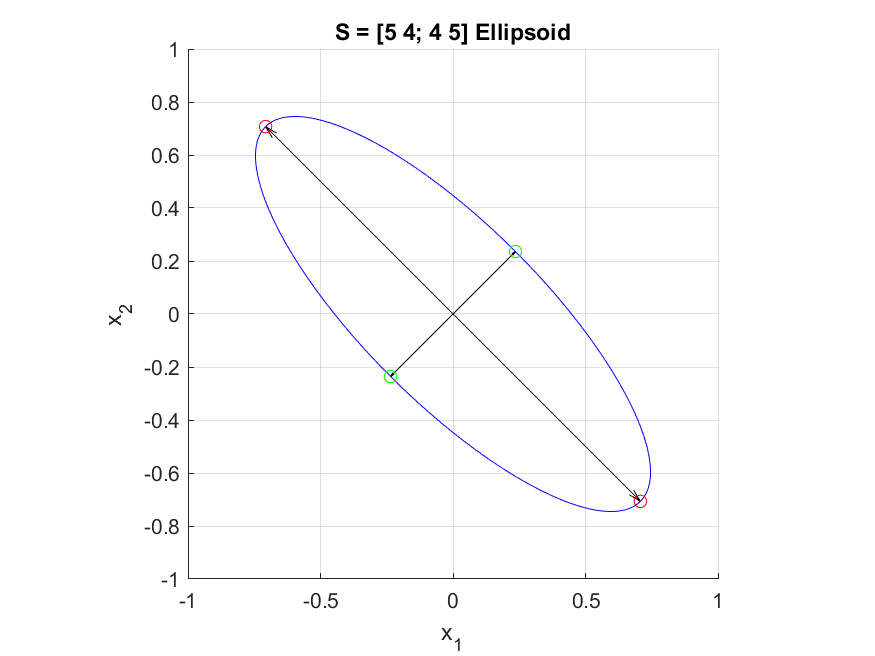
\includegraphics[scale=0.75]{./matlab/chapter-3/sol3.7.1.png}
\end{figure}
\begin{lstlisting}
    S = [5 4; 4 5];
    [V,D] = eig(S);
    MyPlotEllipse(V,D,1,output_path,'sol3.7.1') 
\end{lstlisting}
\[
    \textbf{S}
    =
    \begin{bNiceArray}{cc}
        5 & -4 \\
        -4 & 5
    \end{bNiceArray}
\]
\[
    0
    =
    \left|\textbf{S} - \lambda \textbf{I}\right|
    =
    \left|
    \begin{NiceArray}{cc}
        5 - \lambda & -4 \\
        -4 & 5 - \lambda
    \end{NiceArray}
    \right|
    =
    {(5 - \lambda)}^{2} - 16
    =
    \lambda^2 - 10\lambda + 9
    =
    (\lambda - 9)(\lambda - 1)
\]
The eigenvalues are $\{\lambda_1,\lambda_2\} = \{1,9\}$.
\newline
\underline{$\lambda_1 = 1$:}
\[
    \textbf{S}\textbf{x}_1 = \lambda_1\textbf{x}_1
    \Rightarrow
    \begin{bNiceArray}{cc}
        5 & -4 \\
        -4 & 5
    \end{bNiceArray}
    \begin{bNiceArray}{c}
        x_1 \\
        x_2
    \end{bNiceArray}
    =
    \begin{bNiceArray}{c}
        x_1 \\
        x_2
    \end{bNiceArray}
    \Rightarrow
    \begin{bNiceArray}{cc}
        4 & -4 \\
        -4 & 4
    \end{bNiceArray}
    \begin{bNiceArray}{c}
        x_1 \\
        x_2
    \end{bNiceArray}
    =
    \begin{bNiceArray}{c}
        0 \\
        0
    \end{bNiceArray}
\]
\[
    \textbf{x}_1
    =
    \begin{bNiceArray}{r}
        1 \\
        1
    \end{bNiceArray}
    \Rightarrow
    \textbf{e}_1
    =
    \begin{bNiceArray}{r}
        1/\sqrt{2} \\
        1/\sqrt{2}
    \end{bNiceArray}
\]
\underline{$\lambda_2 = 9$:}
\[
    \textbf{S}\textbf{x}_2 = \lambda_2\textbf{x}_2
    \Rightarrow
    \begin{bNiceArray}{cc}
        5 & -4 \\
        -4 & 5
    \end{bNiceArray}
    \begin{bNiceArray}{c}
        x_1 \\
        x_2
    \end{bNiceArray}
    =
    \begin{bNiceArray}{c}
        9x_1 \\
        9x_2
    \end{bNiceArray}
    \Rightarrow
    \begin{bNiceArray}{cc}
        -4 & -4 \\
        -4 & -4
    \end{bNiceArray}
    \begin{bNiceArray}{c}
        x_1 \\
        x_2
    \end{bNiceArray}
    =
    \begin{bNiceArray}{c}
        0 \\
        0
    \end{bNiceArray}
\]
\[
    \textbf{x}_2
    =
    \begin{bNiceArray}{r}
        1 \\
        -1
    \end{bNiceArray}
    \Rightarrow
    \textbf{e}_2
    =
    \begin{bNiceArray}{c}
        1/\sqrt{2} \\
        -1/\sqrt{2}
    \end{bNiceArray}
\]
Set equal to $c^2$ to have the equation of an ellipse centered at the origin.
\[
    \Rightarrow
    \textbf{x}^{\prime}
    \textbf{S}
    \textbf{x}
    =
    c^2
    =
    \frac{{(\textbf{x}^{\prime}\textbf{e}_1)}^{2}}{{(c/\sqrt{\lambda_1})}^{2}}
    +
    \frac{{(\textbf{x}^{\prime}\textbf{e}_2)}^{2}}{{(c/\sqrt{\lambda_2})}^{2}}
\]
\[
    =
    \frac{{x}_{1}^{2}}{{a}^{2}}
    +
    \frac{{x}_{2}^{2}}{{b}^{2}}
\]
The major axis (related to the smallest eigenvalue) is in the direction of $\textbf{e}_1 = {[(1/\sqrt{2}), (1/\sqrt{2})]}^{\prime}$ with length $a = c/\sqrt{\lambda_1} = 1/1 = 1$.
The minor axis (related to the largest eigenvalue) is in the direction of $\textbf{e}_2 = {[(1/\sqrt{2}), -(1/\sqrt{2})]}^{\prime}$, with length $a = c/\sqrt{\lambda_2} = 1/3$. Here, $c = 1$. This sample covariance matrix, $\textbf{S}$, has the same eigenvalues as the one above, but the eigenvectors here are switched so the major axis is also switched.
\begin{figure}[H]
    \centering
    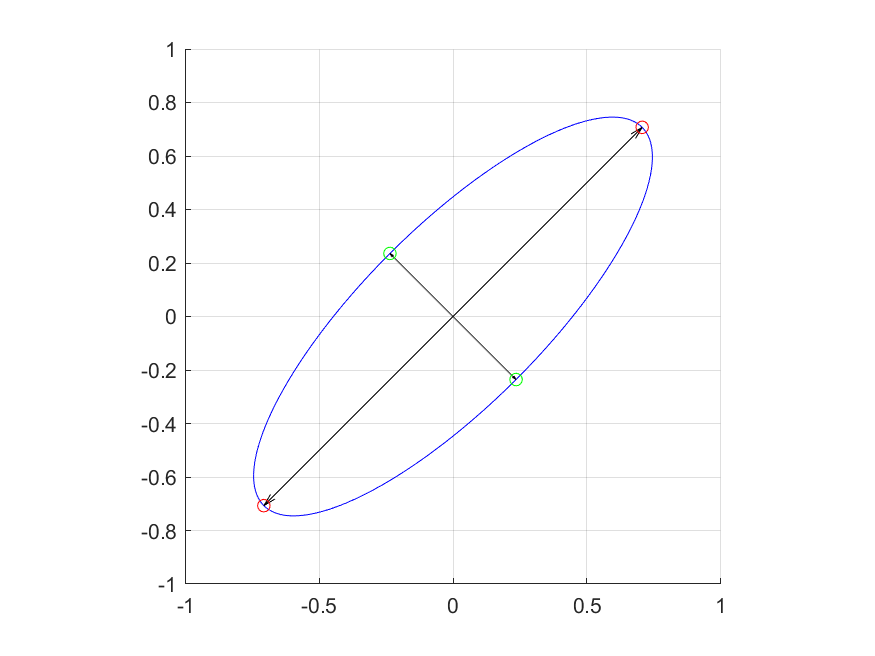
\includegraphics[scale=0.75]{./matlab/chapter-3/sol3.7.2.png}
\end{figure}
\begin{lstlisting}
    S = [5 -4; -4 5];
    [V,D] = eig(S);
    MyPlotEllipse(V,D,1,output_path,'sol3.7.2')
\end{lstlisting}
\[
    \textbf{S}
    =
    \begin{bNiceArray}{cc}
        3 & 0 \\
        0 & 3
    \end{bNiceArray}
\]
\[
    0
    =
    \left|\textbf{S} - \lambda \textbf{I}\right|
    =
    \left|
    \begin{NiceArray}{cc}
        3 - \lambda & 0 \\
        0 & 3 - \lambda
    \end{NiceArray}
    \right|
    =
    {(3 - \lambda)}^{2} - 0
    =
    (\lambda - 3)(\lambda - 3)
\]
The eigenvalues are both 3, $\{\lambda_1,\lambda_2\} = \{3,3\}$.
\newline
\underline{$\lambda_1 = \lambda_2 = 3$:}
\[
    \textbf{S}\textbf{x}_1 = \lambda_1\textbf{x}_1
    \Rightarrow
    \begin{bNiceArray}{cc}
        3 & 0 \\
        0 & 3
    \end{bNiceArray}
    \begin{bNiceArray}{c}
        3x_1 \\
        3x_2
    \end{bNiceArray}
    =
    \begin{bNiceArray}{c}
        3x_1 \\
        3x_2
    \end{bNiceArray}
    \Rightarrow
    \begin{bNiceArray}{cc}
        0 & 0 \\
        0 & 0
    \end{bNiceArray}
    \begin{bNiceArray}{c}
        x_1 \\
        x_2
    \end{bNiceArray}
    =
    \begin{bNiceArray}{c}
        0 \\
        0
    \end{bNiceArray}
\]
Both eigenvalues are the same, so need to pick two vectors. They can be anything, so why not the stand basis vectors for $\R^2$.
\[
    \textbf{x}_1
    =
    \textbf{e}_1
    =
    \begin{bNiceArray}{r}
        1 \\
        0
    \end{bNiceArray}
\]
\[
    \textbf{x}_2
    =
    \textbf{e}_2
    =
    \begin{bNiceArray}{r}
        0 \\
        1
    \end{bNiceArray}
\]
Set equal to $c^2$ to have the equation of an ellipse centered at the origin.
\[
    \Rightarrow
    \textbf{x}^{\prime}
    \textbf{S}
    \textbf{x}
    =
    c^2
    =
    \frac{{(\textbf{x}^{\prime}\textbf{e}_1)}^{2}}{{(c/\sqrt{\lambda_1})}^{2}}
    +
    \frac{{(\textbf{x}^{\prime}\textbf{e}_2)}^{2}}{{(c/\sqrt{\lambda_2})}^{2}}
\]
\[
    =
    \frac{{x}_{1}^{2}}{{a}^{2}}
    +
    \frac{{x}_{2}^{2}}{{b}^{2}}
\]
Here, we have two eigenvalues that are the same, so the lengths in the major and minor axis are also the same. The eigenvectors are the standard basis, so we have a circle centered at the origin with radius $a = b = c/\sqrt{\lambda_1} = 1/\sqrt{3}$. Here, $c = 1$.
\begin{figure}[H]
    \centering
    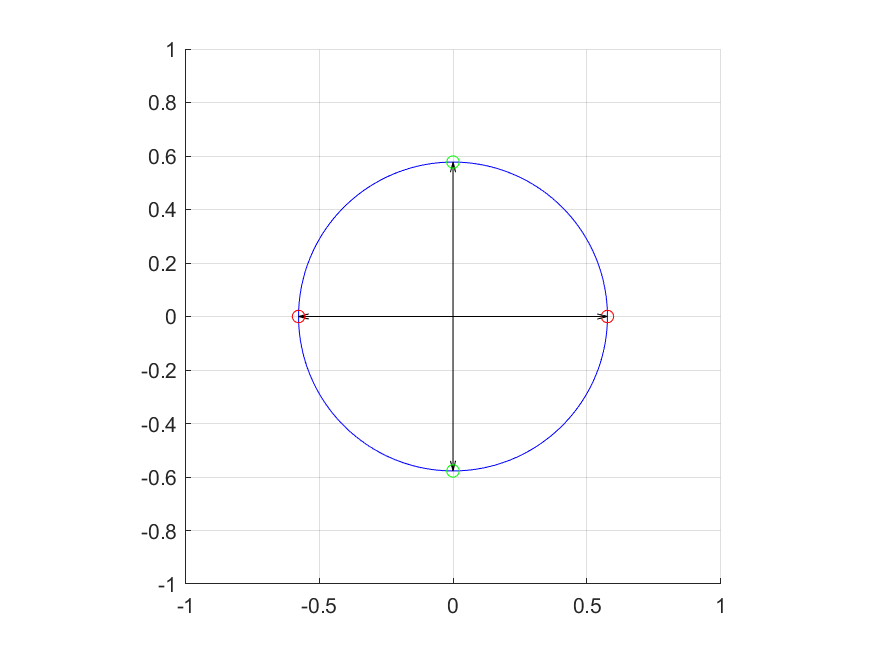
\includegraphics[scale=0.75]{./matlab/chapter-3/sol3.7.3.png}
\end{figure}
\begin{lstlisting}
    S = [3 0; 0 3];
    [V,D] = eig(S);
    MyPlotEllipse(V,D,1,output_path,'sol3.7.3')
\end{lstlisting}